\section{Design and Implementation}
\label{sec:implement}

\NM{} is designed as a replacement for the default memory allocator. It intercepts all memory allocation/deallocation invocations via the preloading mechanism. Therefore, there is no need to change the source code of applications, and there is no need to use custom OS or hardware. Multiple components that differentiate it from existing allocators are further discussed in the remainder of this section.

\begin{figure}[!ht]
\begin{center}
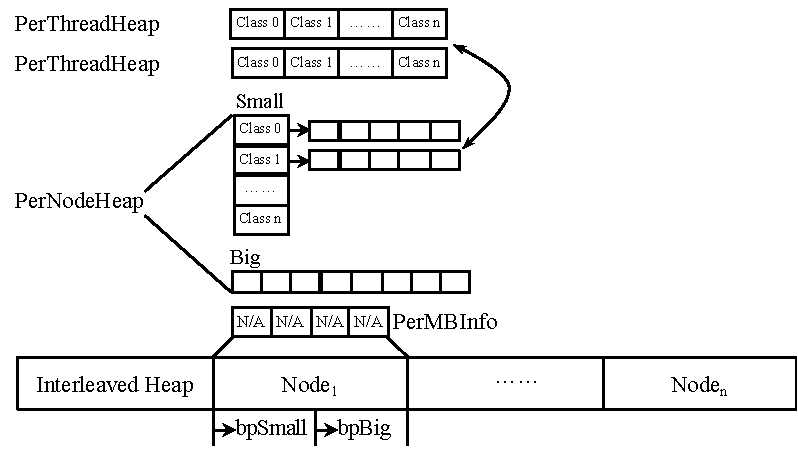
\includegraphics[width=0.45\textwidth]{figure/heaplayout1}
%\includegraphics{figure/overview2}
\end{center}
\vspace{-0.1in}
\caption{Overview of \NA{}'s Heap Layout.
\label{fig:overview}}
\vspace{-0.1in}
\end{figure}

The \NM{}'s heap layout is shown as Figure~\ref{fig:overview}. \NM{} requests a large and continuous region from the underlying OS initially. Then this global region will be divided into multiple regions, which has the same number as  hardware nodes. \NM{} utilizes different mechanisms to manage small and big objects, where objects with the size larger than 512K belongs to big objects. For small objects, \NM{} utilizes the ``\textbf{Bi}g-\textbf{B}ag-\textbf{o}f-\textbf{P}ages'' (BiBOP) mechanism that all objects in the same bag will have the same size class, and separates the metadata from actual objects. Small objects are organized by size classes and will obtain from the \texttt{pbSmall} pointer with the unit of one megabytes. Big objects are always aligned up to megabytes, and tracked by \texttt{pbBig} pointer. Due to this reason, \NM{} maintains the information for each megabytes (with the \texttt{PerMBInfo} structure), which includes the size and the used/free information (with the lowest significant bit). This allows  \NM{} coalesce multiple continuous big objects into a bigger object upon deallocations.  

Each region will be further divided into two sub-regions, one for small objects, and one for big objects. This division allows \NM{} to employ explicit huge pages as discussed in Section~\ref{sec:hugepage}. \NM{} maintains per-thread freelists to track small objects, one for each size class, and one per-node freelist for each node to track big objects. \NM{} also maintains per-node freelists to track small objects based on size classes. These freelists are singly linked lists, which uses the first word of every freed object as pointers.  Small freed objects may be migrated between per-thread freelists and per-node freelists, as further described in Section~\ref{sec: others}. 

\subsection{Origin-Based Memory Management} 
\label{sec:taskassign}

As discussed in Section~\ref{sec:intro}, \NM{} proposes an origin-based memory management, which further includes the following aspects. 

First, it includes an origin-based deallocation, which is the basis of its origin-based allocation. \NM{} proposes node-based freelists to track freed objects that are originated from the current node, and utilizes per-thread freelists to objects freed by the current thread. Differently, a freed object will be \textit{only} placed into its per-thread list if the object is originated from the current node. Otherwise, the object will be placed into its original node's freelist.  

Second, \NM{} includes an origin-computable design as shown in Figure~\ref{fig:overview}, which allows the checking of origin quickly. Basically, the heap is a continuous region that is divided into multiple regions, where each region is bound to a node sequentially via \texttt{mbind} system call. Therefore, given any object, we could compute the physical origin of it by dividing the heap offset with the region size. 

Third, \NM{} always satisfy a memory request of small objects with the following order in order to ensure its origin-computable design and the efficiency: the per-thread's freelist will be checked first, since there is no need to acquire any lock and there is a high chance that the object is still hot in the cache; The current node's freelist will be checked secondly; The last step is to allocate the memory from the current node's un-allocated region, if the last two steps failed. Since the region is bound to the current node and the objects in per-thread freelist and per-node freelist are originated from the current node, \NM{} ensures local allocations. For big objects, freed objects will be tracked in its per-node freelist. Therefore, all allocations will be satisfied from per-node freelist first and then from pbBig pointer (tracking un-allocated region). 

\subsection{Reducing Node Imbalance}
\label{sec:balance}

\NM{} further proposes two mechanisms as follows to reduce node imbalance, where it is the first allocator to implement these mechanisms. 

\paragraph{Node-Balanced Thread Binding} \NM{} proposes a node-balanced thread binding. As described in Section~\ref{sec:intro}, thread migration will cause multiple performance issues for the NUMA architecture. Therefore, \NM{} binds each thread to a node specifically in order to avoid thread migration. To improve the balance, \NM{} binds threads to different nodes in an interleaved way so that every node will have a similar number of threads. The first thread will be bound to the node that it is scheduled to run by the OS. \NM{} only binds a thread to a node, instead of a core, which still allows the load balance initiated by the OS. To perform the binding correctly, \NM{} obtains the hardware topology in the initialization phase via the \texttt{numa\_node\_to\_cpus} API, which tells the relationship between each CPU core and each memory node. Then it intercepts all thread creations in order to bind a newly-created thread to a specific node. 

\paragraph{Interleaved Heap} \NA{} further proposes an interleaved heap. Based on our observation, most NUMA performances issues identified by existing NUMA profilers are related to shared objects that are typically allocated in the main thread~\cite{XULIU, MemProf}. Due to the default first-touch policy~\cite{lameter2013numa, diener2015locality}, objects allocated and touched by the main thread are typically allocated in the first node that the main thread is running on. However, this method could easily cause the load imbalance issue, if such objects are passed to multiple children threads: the memory controller of this node will be accessed by multiple threads concurrently. To overcome this issue, \NA{} reserves a range of memory for such objects, called as ``Interleaved Heap'' in Figure~\ref{fig:overview}. \NA{} utilizes the \texttt{mbind} system call to specify that physical pages of this range will be allocated from all nodes interleavedly. This design helps balance the volume of memory accesses of all memory controllers, reducing interconnect congestion and load imbalance. 

\begin{comment}
\begin{wrapfigure}{r}{0.6\textwidth}
\centering
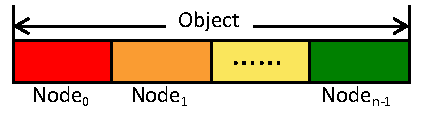
\includegraphics[width=3in]{figure/blockwise}
\vspace{-0.1in}
\caption{Block-wise Memory Allocation\label{fig:blockwise}}
\vspace{-0.1in}
\end{wrapfigure}
\end{comment}

\NA{} should not allocate private objects from the interleaved heap, since that will create remote accesses unnecessarily. For this purpose, \NM{} should be able to differentiate shared objects from private objects. Although programmers could provide such information, that will require the change of programs or manual intervention. Instead, \NM{} utilizes a simple heuristics to identify potentially-shared objects, based on allocation callsites: each allocation callsite is treated as a shared one initially, and is allocated from the interleaved heap; When an object is deallocated before creating children threads, all objects from the corresponding callsite are considered to be private ones, and then are only allocated from the per-node heap afterward. 

 \NM{} monitors allocation/deallocation pattern to identify the share-ability of each callsite. For the performance reason, \NA{} further utilizes the sum of the stack position and the return address of the allocation to identify a callsite, called ``\textit{callsite key}'', instead of using the slow \texttt{backtrace}~\cite{DBLP:conf/icse/SumnerZWZ10, DBLP:conf/cgo/ZengR0AJ014}. This combination is able to differentiate callsites correctly if an application does not have allocation wrappers, since stack positions can be utilized to identify the number of functions in the stack and the return address tells the invocation placement inside the same function. If a callsite is mis-identified, it won't cause any correctness issue, but with some performance penalties. For the performance reason, \NA{} utilizes a hash table to track the status of every callsite.
 % which is fortunately not very expensive given the limited amount of different callsites. 
 

%\NM{} requires to track the shared pattern for each callsite. For the performance reason, \NA{} further proposes to utilize the sum of the stack position and the return address of the allocation to identify a callsite, called ``\textit{callsite key}''. When memory allocations are invoked in different functions, their stack positions are likely to be different. The return address (of the application) tells the invocation placement inside the same function. However, this design cannot completely avoid mis-identification issue,  where multiple allocations inside the allocation wrapper will be treated as the same callsite. However, the mis-identification will not cause any correctness issue, but only performance issue. During the implementation, we have thought about two other mechanisms. One is to obtain the callsite correctly with the \texttt{backtrace} function, but it is too slow to be used in production environment. The other mechanism will require the recompilation to encode calling context explicitly~\cite{DBLP:conf/icse/SumnerZWZ10, DBLP:conf/cgo/ZengR0AJ014}.
  
%   A shared callsite can be treated as a private callsite, if an object from  these callsites invokes the deallocation before creating children threads. For the performance reason, \NA{} obtains the return address quickly via a constant offset, where the offset is uniquely determined after the compilation of \NA{}. 

%\NA{} utilizes a hash table to track the status of every callsite. Upon every allocation of the main thread, \NA{} checks the status of the allocation callsite, with the callsite key as described above. If the callsite is identified as a shared callsite, the current allocation will be satisfied from the interleaved heap. Otherwise, it will be allocated from the per-node heap. Upon deallocations, \NM{} marks an allocation callsite as private, if an object from this callsite has been deallocated before creating other threads. 

%When an allocation is satisfied in the callsite and the callsite is new, the corresponding allocation will be tracked in the second hash table. The second hash table will be checked upon deallocations, where the corresponding allocation callsite will be marked as private if an object is allocated in the same epoch. 

\subsection{Explicit Huge Page Support} 
\label{sec:hugepage}

 Based on the existing study~\cite{hugepages}, huge pages can reduce Translation Look-aside Buffer (TLB) misses, and reduce the interferences on the cache utilization caused by TLB misses (and thus cache misses). However, existing  transparent huge page support is not good for the performance~\cite{Gaud:2014:LPM:2643634.2643659, DBLP:conf/asplos/PanwarBG19}, due to hot page effect, page-level false sharing, and increased memory footprint~\cite{DBLP:conf/asplos/MaasAIJMR20}.
 
\NA{} proposes explicit huge pages to avoid these issues, by choosing which objects should be allocated from huge pages carefully. If huge pages are only utilized for private objects for threads running on the node, then there is no hot page effect and page-level false sharing. Also, if huge pages are only utilized for big objects that are larger than the page size, then there is no need to worry about unnecessary memory consumption. Based on these observation,  \NM{} only employs huge pages for large objects with the size larger than a huge page, and for small objects that are predicted to be allocated frequently. For the latter one, \NM{} employs the history information to predict, and only uses huge pages for a size class that has used at least one bag before. 

%In addition to large objects that has the size larger than the size of a huge page, huge pages are only utilized for small objects that are predicted to be used a lot.  \NA{} employs the history of memory allocation to predict this. 
%Each per-node heap is further divided into two parts as illustrated in Figure~\ref{fig:overview}: small objects will be allocated from the first half and will be allocated using small pages, while big objects will be allocated from the second half with huge pages (2MB). When a big object (with the huge page) is utilized for small objects, only frequently-allocated small objects can utilize such an object. We believe that our design balances the performance and memory consumption.   

\subsection{Other Mechanisms}
\label{sec: others}

\NM{} also implements the following mechanisms in order to reduce the performance and memory overhead. 

\paragraph{Efficient Object Migration} Freed objects will be migrated frequently between per-thread and per-node freelists. On the one hand, when a per-thread freelist has too many objects, some should be moved to the per-node freelist so that other threads could re-utilize these freed objects, reducing memory blowup~\cite{Hoard}. On the other hand, each per-thread list needs to obtain freed objects from its per-node heap, when a thread is running out of the memory. Therefore, an efficient mechanism is required to support frequent migration. 

%\NM{} utilizes singly link lists to manage freed objects, imposing an additional challenge of migrating objects efficiently. 

A straightforward method is to traverse the freelist to collect a specified number objects, and then moves all of them at a time in order to reduce the synchronization overhead. Both TcMalloc and TcMalloc-NUMA utilize this mechanism, which has the following issues. First, traversing the freed objects of a freelist will actually bring the first lines of each object to the cache, since the first word of each freed object is used as the pointer for the freelist. This traverse will pollute the cache of the current thread, especially when a thread is moving these objects out. 
%\NM{} utilizes the first word of each freed object as the pointers for the linked list, where traversing these objects will bring these objects to the cache that the current thread do not need. 
Second, the migration will always migrate recently-freed objects, due to the use of singly-link list. This method is not good for the performance when moving objects from a per-thread freelist to the per-node freelist, since recently-freed objects are still hot in the cache. 
Third, the traverse of a global freelist may introduce significant lock contention, when multiple threads are migrating freed objects from the per-node freelist concurrently.
% We observed  20\% slowdown for some applications, due to this straightforward mechanism. \NM{} further proposes an efficient mechanism to migrate objects efficiently. 

\begin{figure}[!h]
\centering
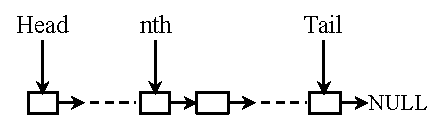
\includegraphics[width=3in]{figure/perthreadlist}
\vspace{-0.1in}
\caption{Avoiding the traverse of per-thread freelist\label{fig:perthreadlist}}
\vspace{-0.1in}
\end{figure}

\NM{} proposes the following data structures to avoid these issues. First, each per-thread freelist maintains two pointers that pointing to the least recent object (shown as the \texttt{Tail} pointer) and the $nth$ object separately (shown as $nth$), as shown in Figure~\ref{fig:perthreadlist}. Each freelist has a header pointer pointing to the most recent object, shown as \texttt{Header}, which will be updated upon adding or deleting an object. This structure avoids the traverse of freelist during the migration, and allows the movement of the least-freed objects (between $(n+1)th$ and $Tail$) to the per-node freelist. After the migration, the \texttt{Tail} pointer will be set to the original $nth$ object. 

%\Maintaining the pointer to the $nth$ object requires only a forward traverse to obtain the pointer of $(n-1)th$ object, and then a thread can migrate $n$ objects (between $(n-1)th$ and the \texttt{Tail} object) easily. 
%After the migration,  the \texttt{Tail} pointer can be set to the original $nth$ object. However, this mechanism alone cannot reduce the lock contention when multiple threads are concurrently obtaining objects.

\begin{figure}[!ht]
\centering
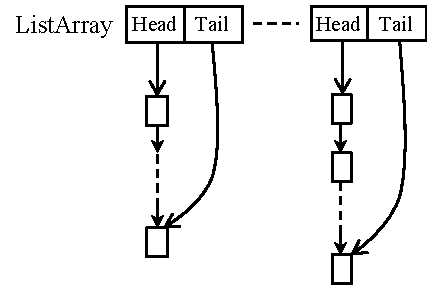
\includegraphics[width=3in]{figure/listarray}
\caption{An array of freelists for per-node heap\label{fig:listarray}}
\vspace{-0.1in}
\end{figure}

Second, \NM{} avoids the bottleneck of the per-node freelist with a circular array as shown in Figure~\ref{fig:listarray}. Each entry of the circular array has two pointers, \texttt{Head} and \texttt{Tail} separately. Each per-node freelist has three types of operations that can be greatly reduced with this data structure. First, a remote thread will put a freed object into the freelist, based on the origin-based deallocation. This operation can be done in a constant time, by putting the object into the entry pointed by a \texttt{toPut} pointer. Second, a local thread maybe put multiple objects into it, which can be finished in constant time as well. All objects will be putted to the entry pointed by a \texttt{toPut} pointer, and then the pointer will be updated to the next entry. Third, the operations for getting objects from it can be done efficiently by simply move all objects in the current entry, since there is no need to traverse the freelist. Therefore, this data structure reduces the synchronization issue of all operations. 
%In order to support the put and get operations to the freelist, this array has two pointers, \texttt{toGetIndex} and  \texttt{toPutIndex}. If a thread tries to obtain freed objects from the per-node heap, it will obtain all  objects pointed by the \texttt{toGetIndex}, and increment the index afterward. If the freelist pointed by the \texttt{toGetIndex} has no freed objects, there is no freed objects in the per-node freelist for this size class.  The put operation will utilize the pointer \texttt{toPutIndex}. There are two scenarios for the put operation. 
%First, a thread may put an freed object directly to the per-node freelist, if this object is originated from a different node that the thread does not belong to. In this case, the object will be placed into the freelist pointed by the \texttt{toPutIndex}, but the index is not updated after the deallocation. Second, when freed objects in a per-thread freelist is above the predefined watermark, the thread will migrate a batch of objects to the freelist pointed by the \texttt{toPutIndex}. After this migration, the current freelist is considered to be full, and will update the index to the next entry in the circular array.

\paragraph{Node-Local Metadata:} \NM{} guarantees that all of the metadata is always allocated in the same node, based on its thread binding as described in Section~\ref{sec:taskassign}. Such metadata includes per-node and per-thread freelists for different size classes, and freelists for big objects. Similarly, \NM{} utilizes the \texttt{mbind} system call to bind the memory to a specific node.  

\paragraph{Reducing Memory Consumption:} \NM{} utilizes multiple mechanisms to reduce the memory consumption. First, if a thread exits, then all memory will be utilized by a new thread. Second, \NM{} reduces the memory overhead when huge pages are employed.  For the latter case, \NM{} makes multiple threads share the same bag (for the same size class), instead of having a separate bag for each thread. If a thread is running out of the memory, it obtains multiple objects at a time from the corresponding bag, instead of getting a separate bag. Based on our evaluation, this mechanism reduces most of memory consumption, with the transparent huge page support by default.  

 %every thread has its own freelists for each size class so that there is no need to acquire the lock when an allocation can be satisfied from its per-thread heap, similar to TcMalloc. That is, two threads will not share the same per-thread heap. However, some applications may create new threads after some threads have exited. \NM{} re-utilizes the memory for these exited threads. Basically, \NM{} intercepts thread joins and cancels so that it can assign heaps of exited threads for newly-created threads, and re-utilize their heaps correspondingly.  


%\paragraph{Transparent Huge Page Support:} During the development, we noticed that excessive memory consumption can be imposed when the OS enables transparent huge pages by default. In order to reduce memory consumption, \NM{} makes multiple threads share the same bag (for the same size class), instead of having a separate bag for each thread. If each thread is running out of the memory, it obtains multiple objects at a time from the corresponding bag. Currently, if a class size is less than one page, then we will at most get objects with the total size of one normal page. Otherwise, it will get 4 objects (with the size less than 64 KB) or 2 objects afterward. Based on our evaluation, this mechanism actually reduces the memory consumption for multiple times for a machine with 128 cores and 8 nodes, with the transparent huge page support by default.  

\paragraph{Cache Warmup:} \NM{} also borrows the cache warmup mechanism of TcMalloc~\cite{tcmalloc}: it will insert all objects in a page into the freelists, if there is no objects in the per-thread freelist. We believe that inserting multiple objects into the freelist will benefit data prefetches, since the insertion is a simple and predictable pattern. With this mechanism, \texttt{raytrace} improves the performance by 10\%. However, this is the only application that we observed such performance improvement. 

%TcMalloc utilizes a \texttt{mmap} system call to obtain multiple pages (depending on the class size) from the OS each time, when it is running out of the memory for one size class. For such a memory block, TcMalloc inserts all objects of this block into its central freelist at one time. Since TcMalloc utilizes the first word of each object as the pointer for the freelist, this mechanism warms up the cache by referencing the first word of each object during the insertion. According to our observation, this warmup mechanism improves the performance of one application (\texttt{raytrace}) by 10\%. Based on our understanding, the performance improvement is caused by data prefetches, since inserting objects to the freelist has a simple and predictable pattern. \NM{} employs a similar mechanism for small objects with the size less than 256 bytes, and adds all objects inside a page to the per-thread freelist. 

%we propose the combination of per-node heap and per-thread cache. In order to reduce the contention, \NM{} will obtain multiple objects at a time from the per-node heap. 

 
%https://queue.acm.org/detail.cfm?id=2852078

